\newpage\section{Evaluation of the solution}

To validate the developed prototype, the previously established test cases are verified for the individual requirements. The testing of the test cases provides information about the degree of fulfillment of the requirements. In addition, the fulfillment of requirements that could not be validated by test cases is considered. Subsequently, the usability of the \ac{ui} of the prototype is assessed.

\subsection{Prototype validation}
This section looks at the individual test cases from Section \ref{subsec:requirement_validation} and describes both their implementation and the degree to which they have been fulfilled. Furthermore, the fulfillment of requirements that cannot be confirmed by test cases is evaluated. 

\newpage\subsubsection*{T1: A welcome and goodbye message is displayed} 

The implementation of this test case can be done without further development by utilizing the standard functionalities of the developed prototype. For this purpose, the Information Screen Activity is specified as the first and last step in the experiment data. Furthermore, a corresponding welcome and farewell text is stored in the experiment data. Figure \ref{fig:T1} shows that the functional requirements F1.1 and F2.1 to show information at the beginning of the experiment and to provide the participants with debrifing information can be completely fulfilled by the artefact.

\vspace{1.5cm}

\begin{figure}[htbp]
    \centering
    \begin{subfigure}[b]{0.25\textwidth}
        \centering
        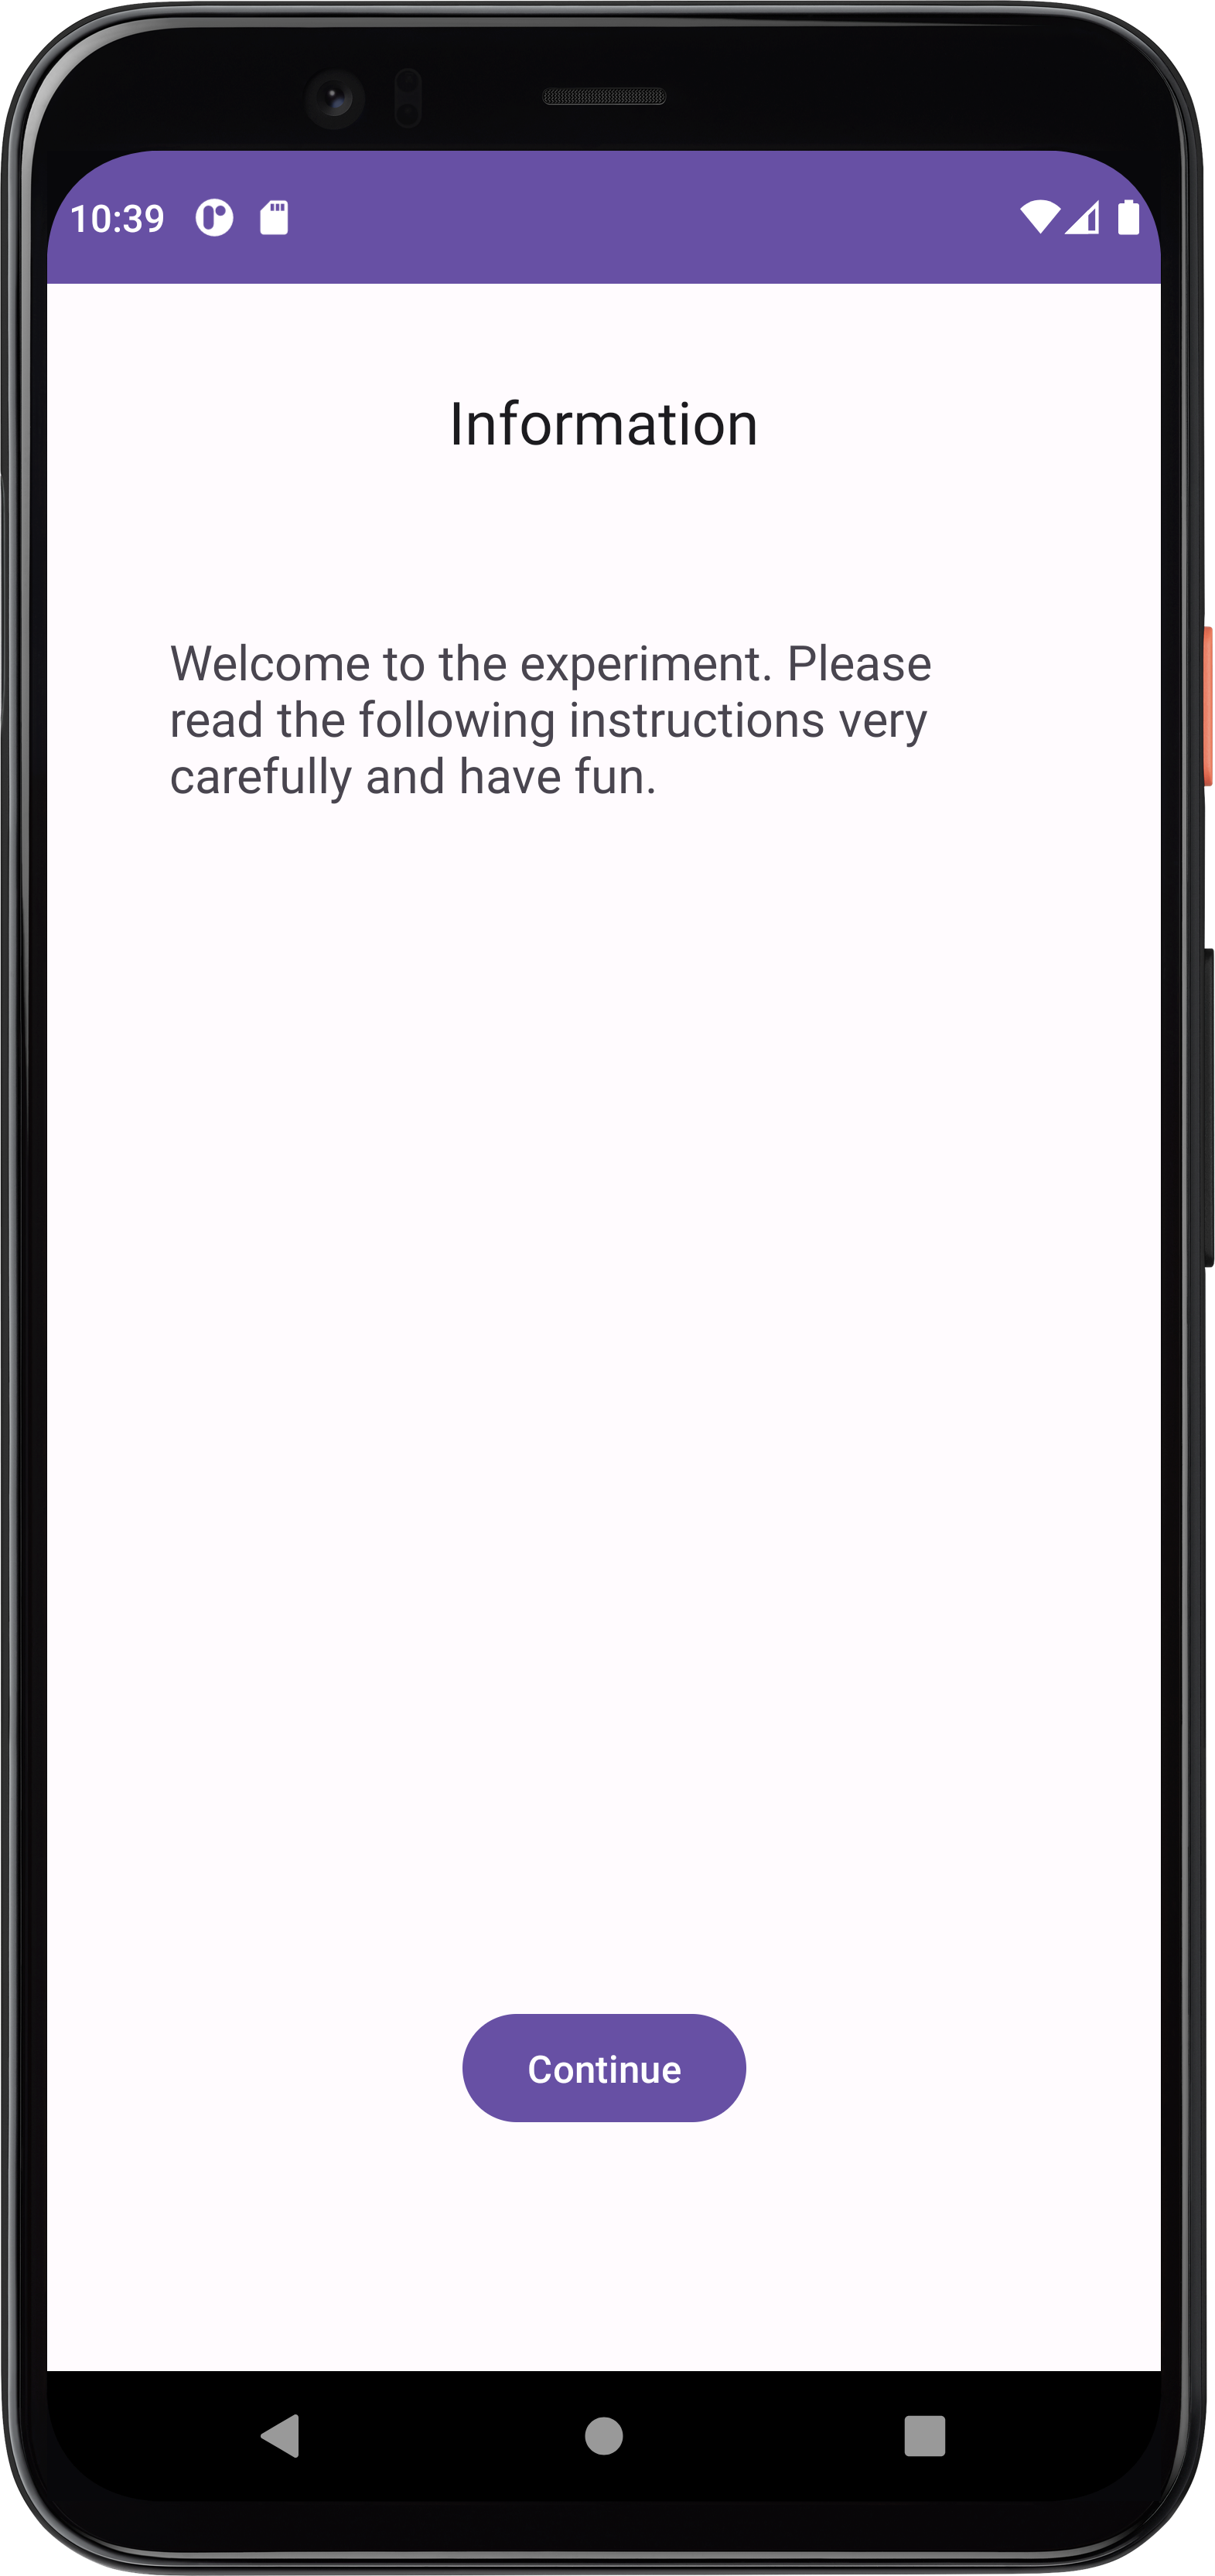
\includegraphics[width=\textwidth]{content/07_evaluation_of_the_solution/Screenshot_StartingScreen.png}
        \caption{Welcome Message}
        \label{subfig:welcomeMessage}
    \end{subfigure}
    \hspace{1cm}
    \begin{subfigure}[b]{0.25\textwidth}
        \centering
        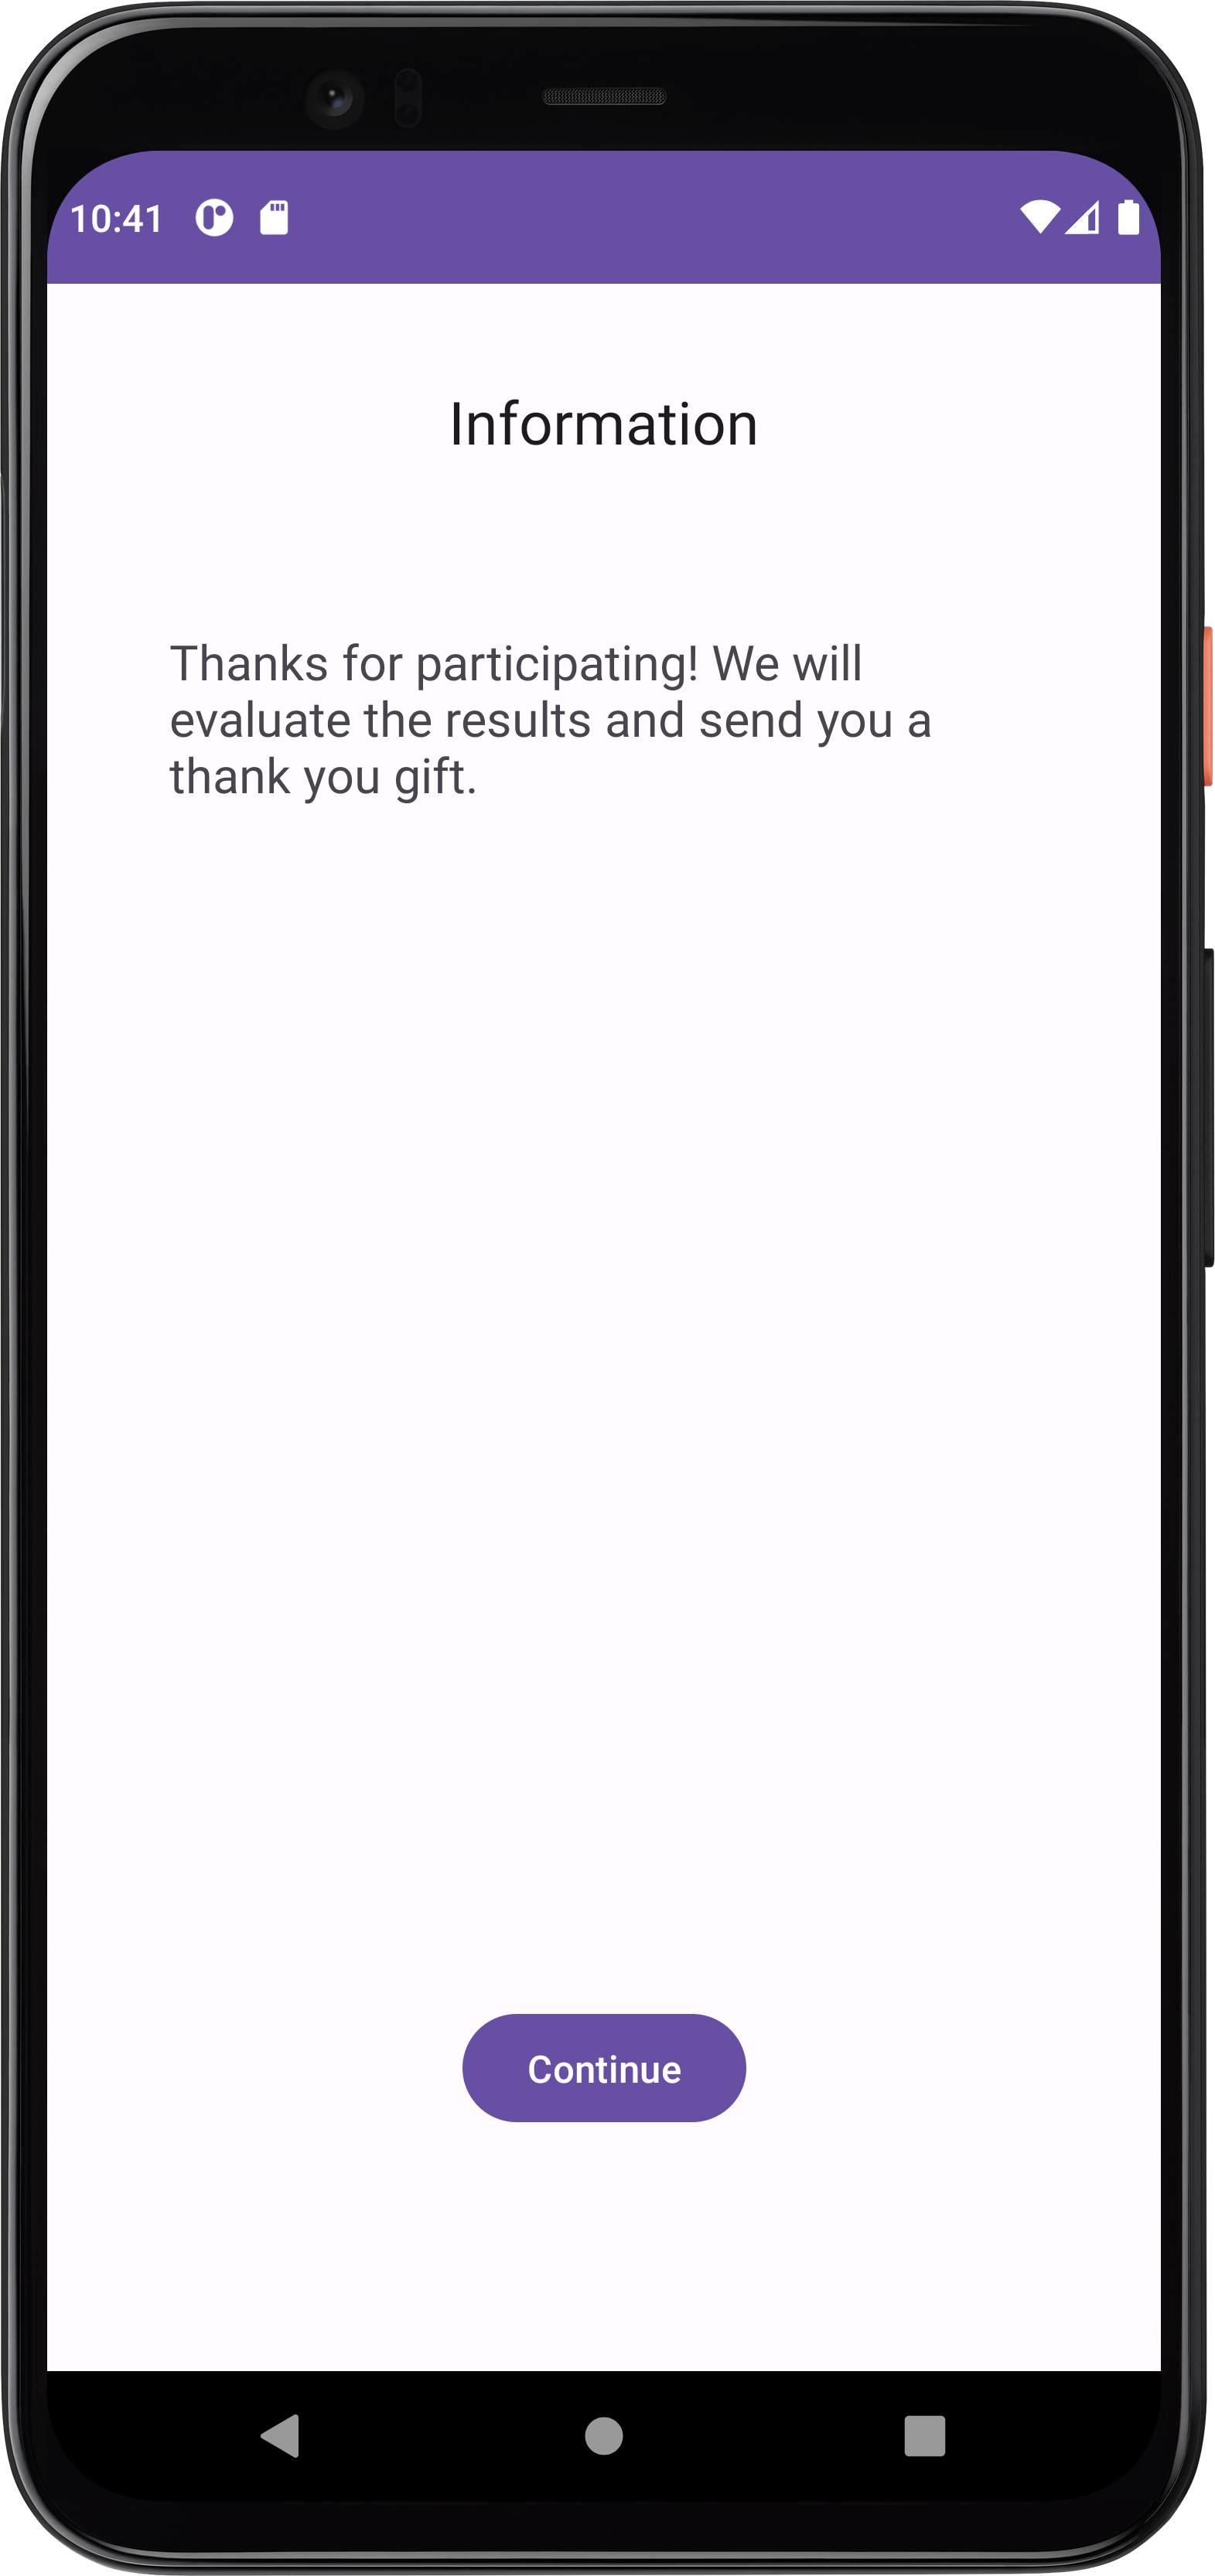
\includegraphics[width=\textwidth]{content/07_evaluation_of_the_solution/Screenshot_GoodbyeMessage.png}
        \caption{Goodbye Message}
        \label{subfig:goodbyeMessage}
    \end{subfigure}
    \caption{User Interface Testcase T1}
    \label{fig:T1}
\end{figure}

\newpage\subsubsection*{T2: Participants are prompted to input their age at the beginning and prompted to input how the liked the experiment at the end}

To perform this test, the experiment data must also be adjusted first. For this, the questionnair step must be placed at the beginning and the end of the experiment steps order within the experiment data. In addition, the participant data must contain the respective data to be queried as an attribute which must not be filled, since the query of the questionnair process only queries for missing data. These data entries are \enquote{age} and \enquote{experiment feedback} as defined by the test case. The two screens on which the participants are asked for their age at the beginning of the experiment and for feedback on the experiment at its end are shown in Figure \ref{fig:T2}. The test T2 and thus the requirements F2.1, F2.3, F2.2 and F2.3 can thus be fulfilled.

\vspace{0.5cm}

\begin{figure}[htbp]
    \centering
    \begin{subfigure}[b]{0.25\textwidth}
        \centering
        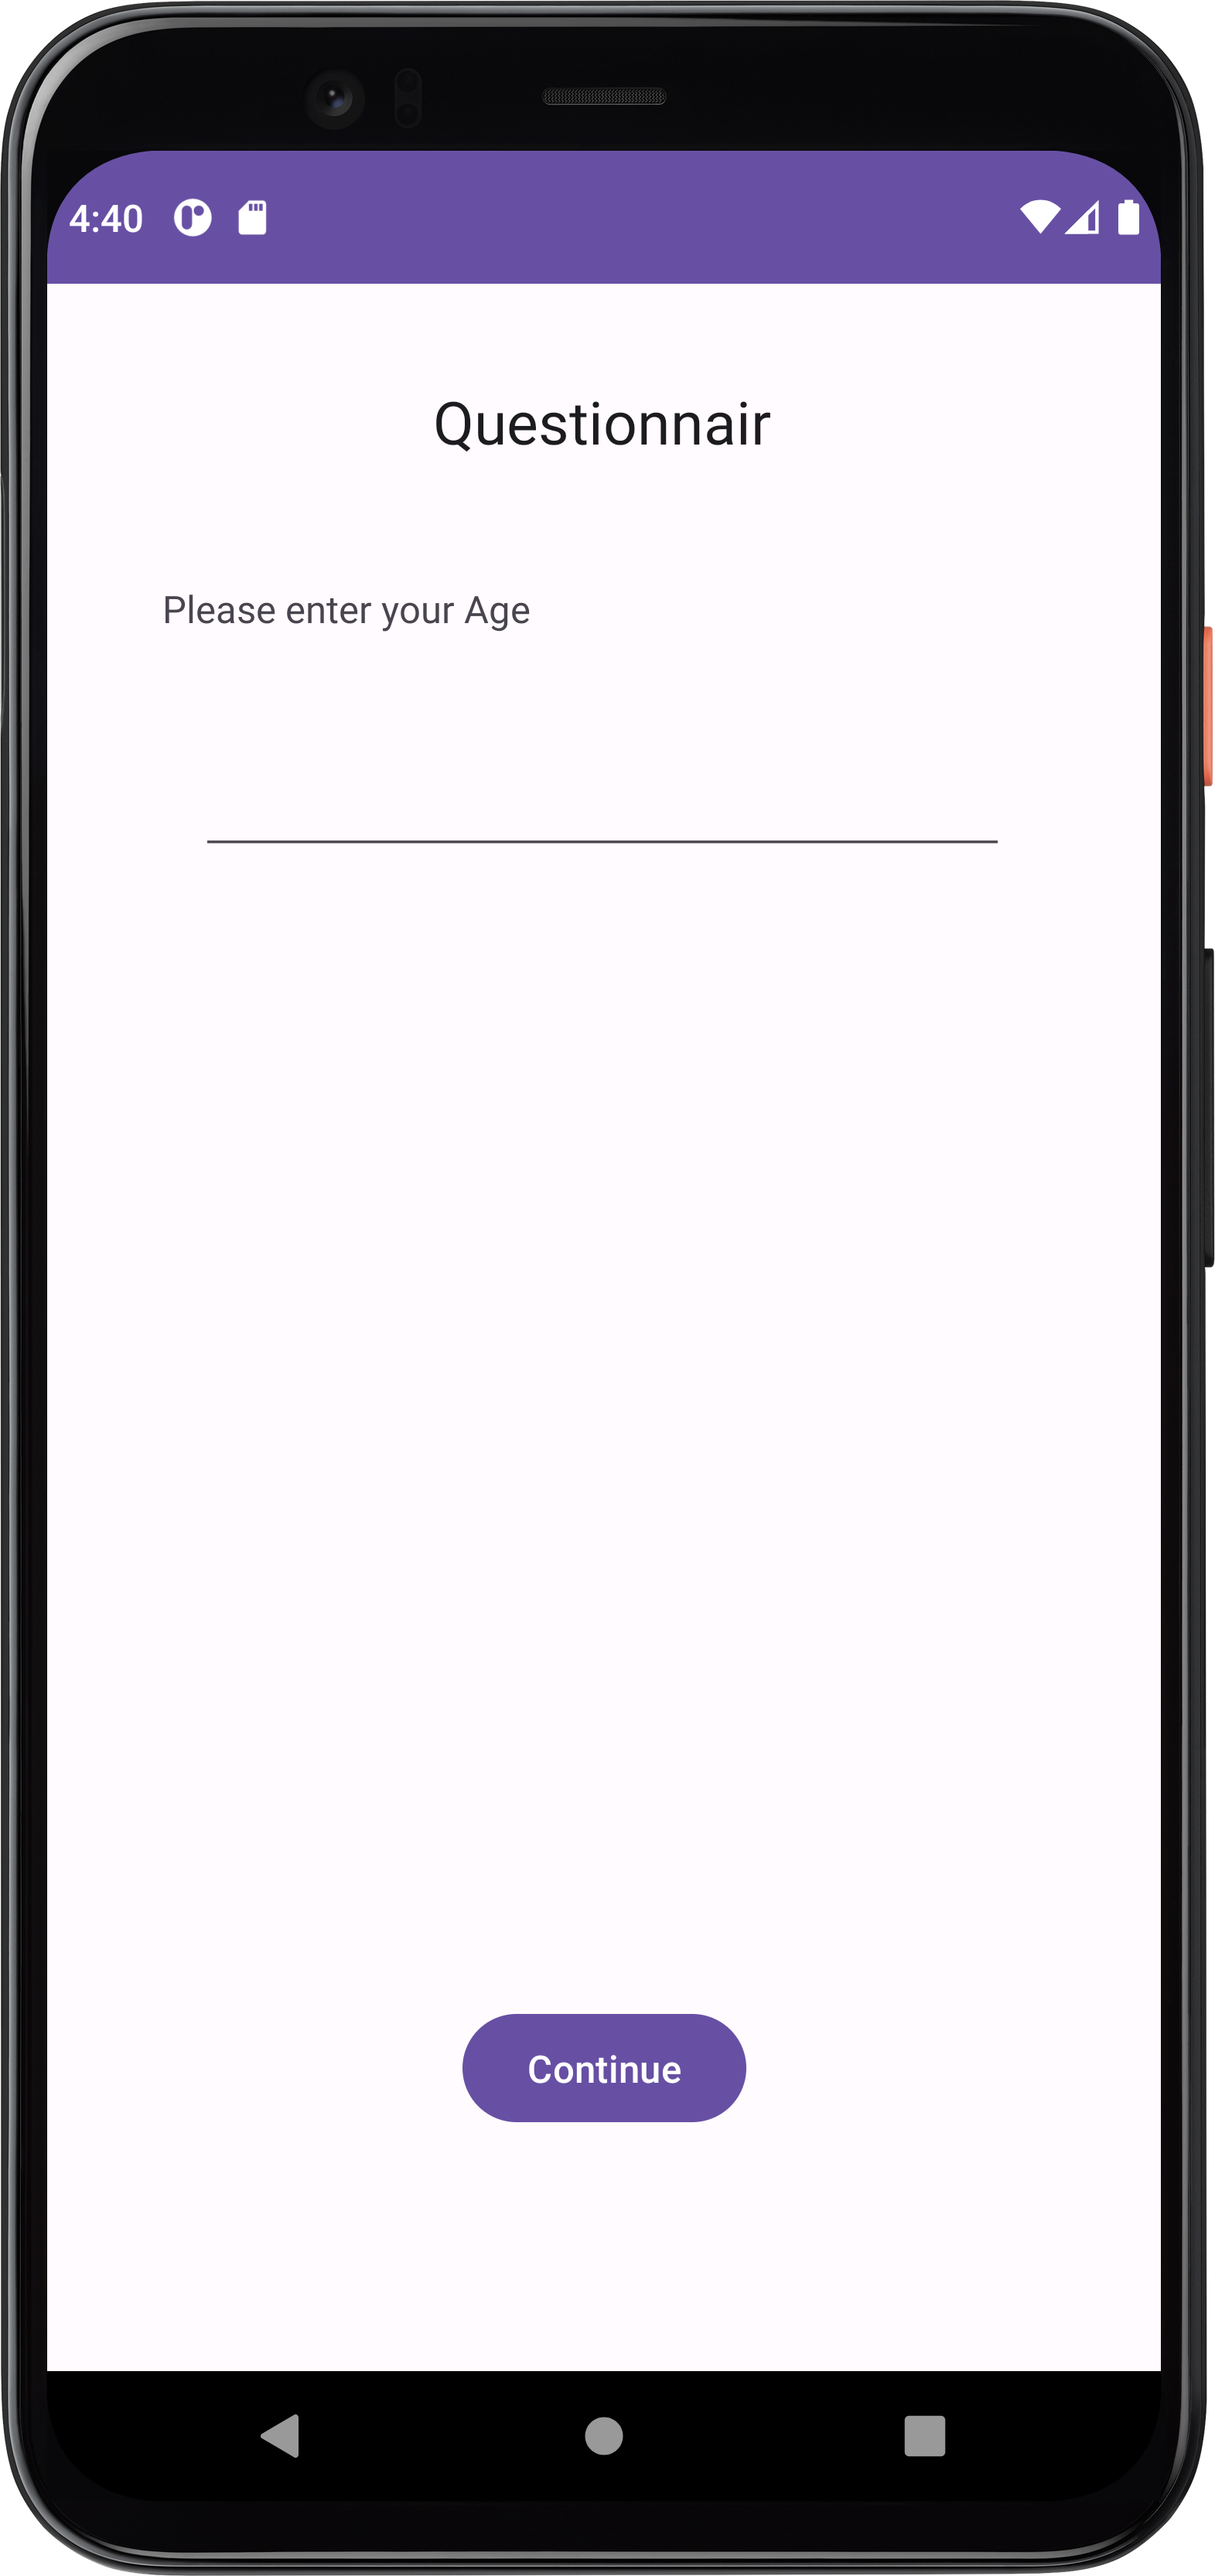
\includegraphics[width=\textwidth]{content/07_evaluation_of_the_solution/Screenshot_T2a.png}
        \caption{Welcome Message}
        \label{subfig:t2a}
    \end{subfigure}
    \hspace{1cm}
    \begin{subfigure}[b]{0.25\textwidth}
        \centering
        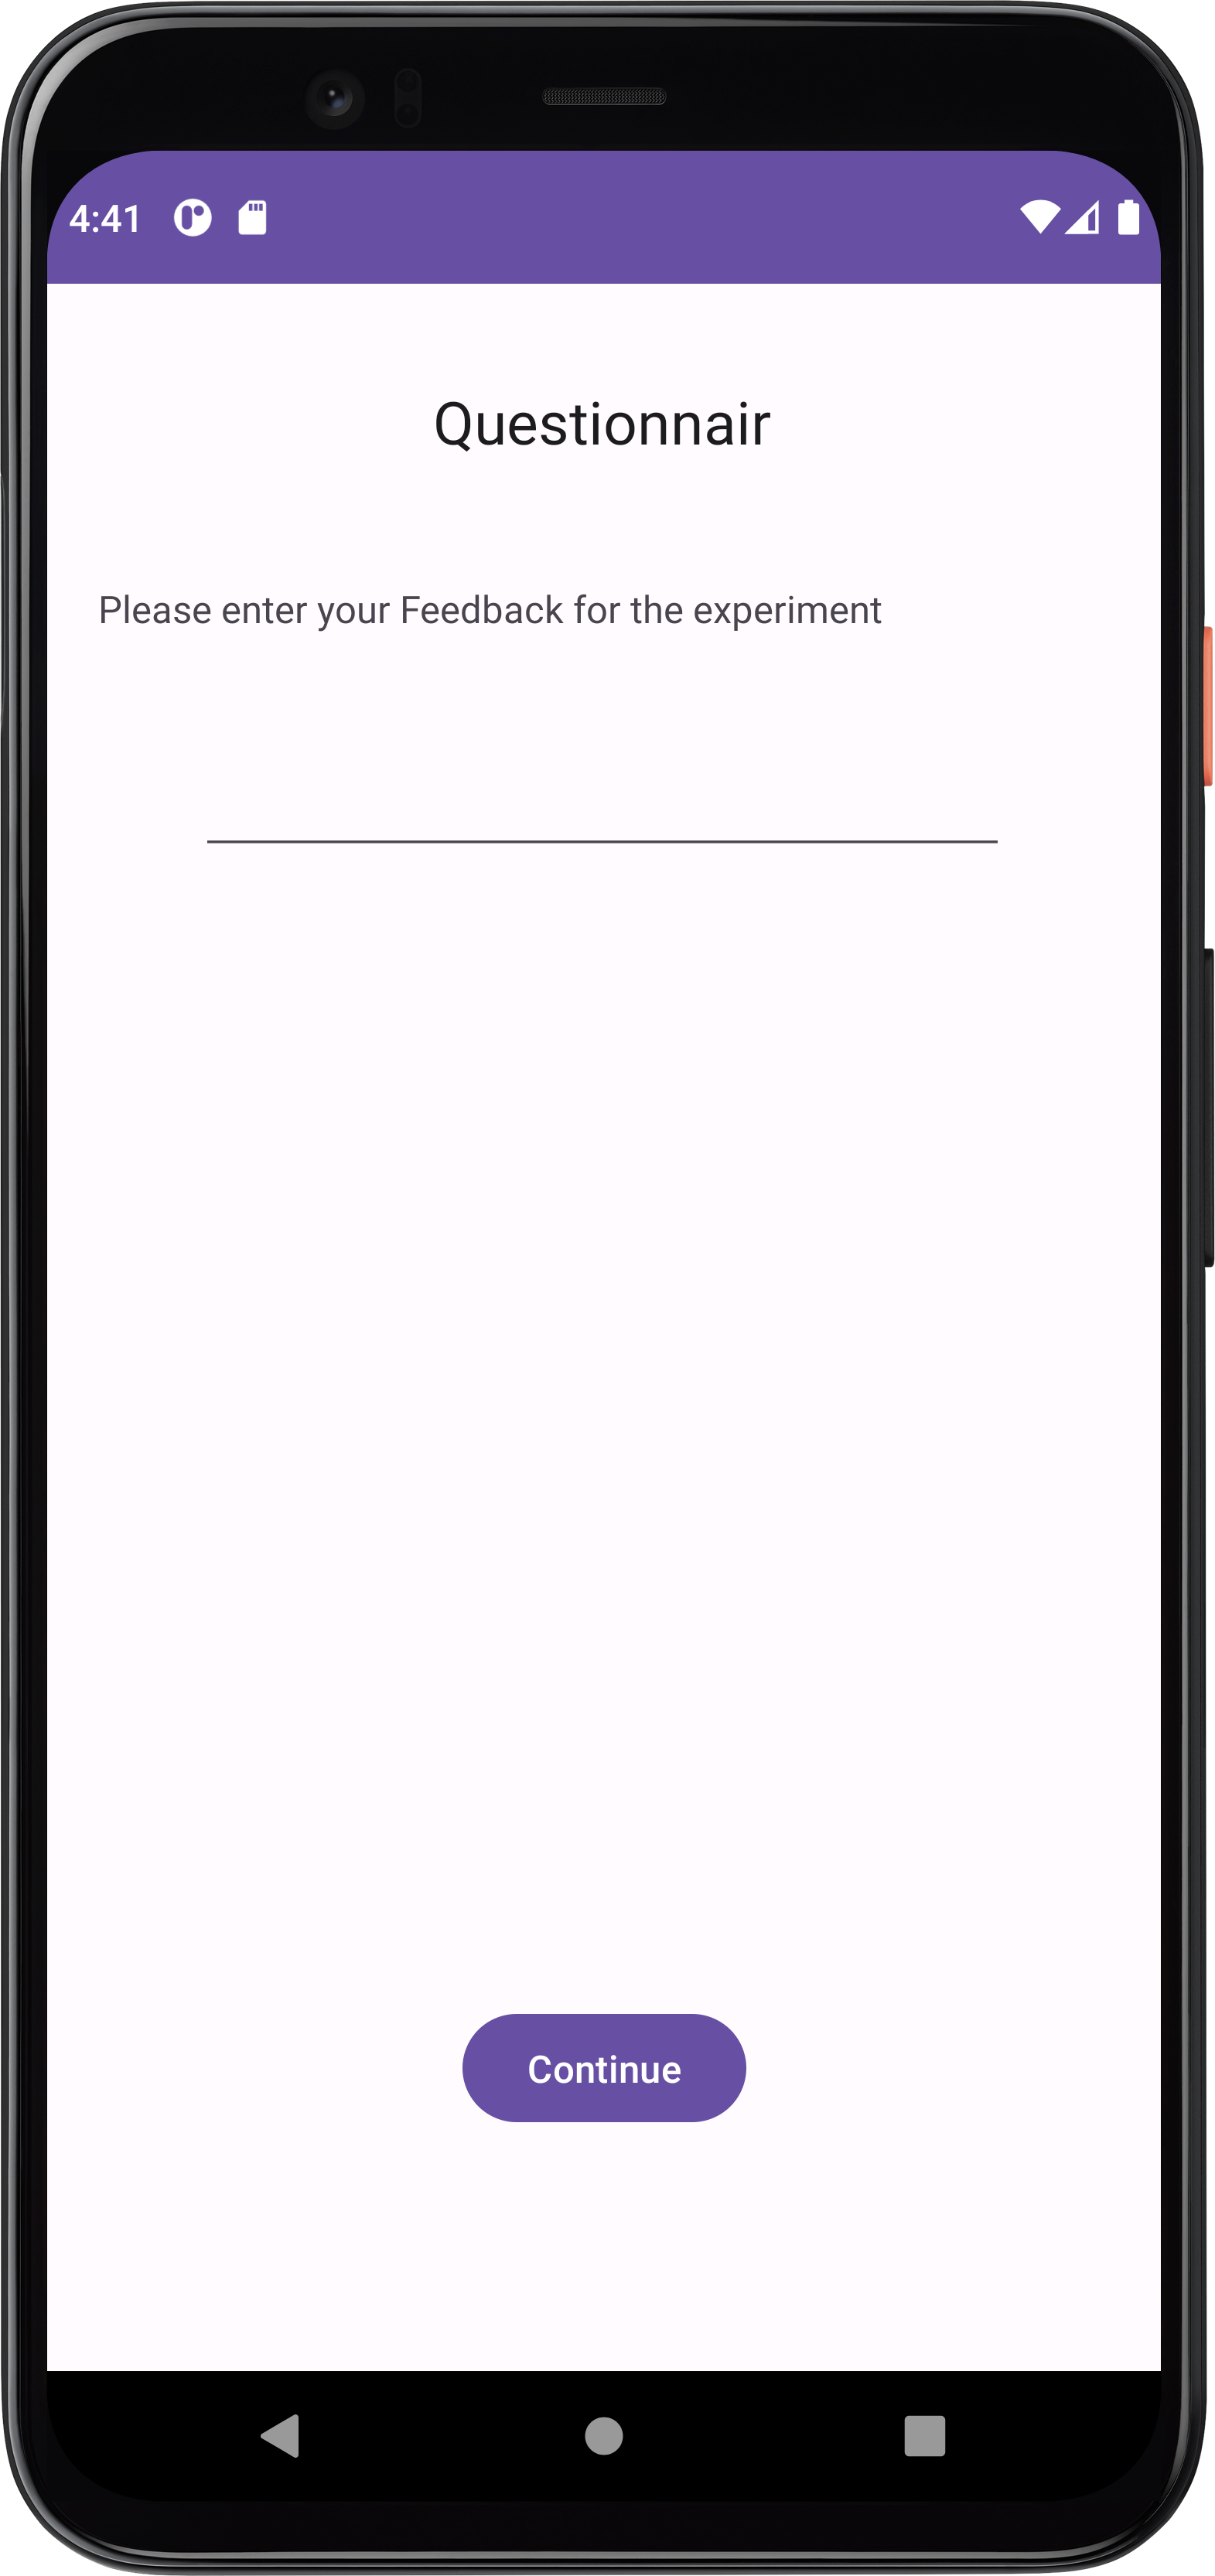
\includegraphics[width=\textwidth]{content/07_evaluation_of_the_solution/Screenshot_T2b.png}
        \caption{Goodbye Message}
        \label{subfig:t2b}
    \end{subfigure}
    \caption{User Interface Testcase T1}
    \label{fig:T2}
\end{figure}

\newpage\subsubsection*{T3: The information about how long the experiment took is collected}

To fulfill this test case, which checks requirement F2.2, the time necessary to perform the experiment is measured. For this, the lines of code from Listing \ref{t3a} can be used on the start activity. These store the start time of the experiment in the meta data in the experiment data. The experiment is then run and the code lines in Listing \ref{t3b} are called when the experiment is completed. These code lines retrieve the start time of the experiment from the experiment data and calculate the total elapsed time during the experiment using the current system time. This is then also stored in the meta data of the experiment data. Thus, the test case T3 can be completely fulfilled and consequently the requirement F2.2.

\vspace{1cm}

\begin{lstlisting}[language=java,label=t3a,lineskip={0pt}, caption=Collect time needed to conduct experiment (a), basicstyle=\scriptsize, captionpos=b]
    String currentTime = new SimpleDateFormat("HH:mm:ss", Locale.getDefault()).format(new Date());
    LogMetaDataUseCase.getInstance().setMetaData(currentTime);
\end{lstlisting}

\begin{lstlisting}[language=java,label=t3b,lineskip={0pt}, caption=Collect time needed to conduct experiment (b), basicstyle=\scriptsize, captionpos=b]
    long difference = date1.getTime() - date2.getTime();
    LogMetaDataUseCase.getInstance().setMetaData(difference);
\end{lstlisting}


\newpage\subsubsection*{T4: The gender and the weight of the participant is pre-loaded into the experiment from different files. The gender of the participant is deleted}

\vspace{1cm}

\begin{lstlisting}[language=java,label=t3b,lineskip={0pt}, caption=Collect time needed to conduct experiment (b), basicstyle=\scriptsize, captionpos=b]
    File csvfile = new File(Environment.getExternalStorageDirectory() + "/participantData.csv");
    CSVReader reader = new CSVReader(new FileReader(csvfile.getAbsolutePath()));
    String[] nextLine;
    while ((nextLine = reader.readNext()) != null) {
        // nextLine[] is an array of values from the line
        ParticipantEntity participant = new ParticipantEntity(Integer.parseInt(nextLine[0]));
        participant.setName(nextLine[0]);
        participant.setEducation(nextLine[0]);
        participant.setGender(null);
    
        data.add(participant);
    }
\end{lstlisting}

\newpage\subsubsection*{T5: A chess game is added as custom logic}

\vspace{1.5cm}

\begin{figure}[htbp]
    \centering
    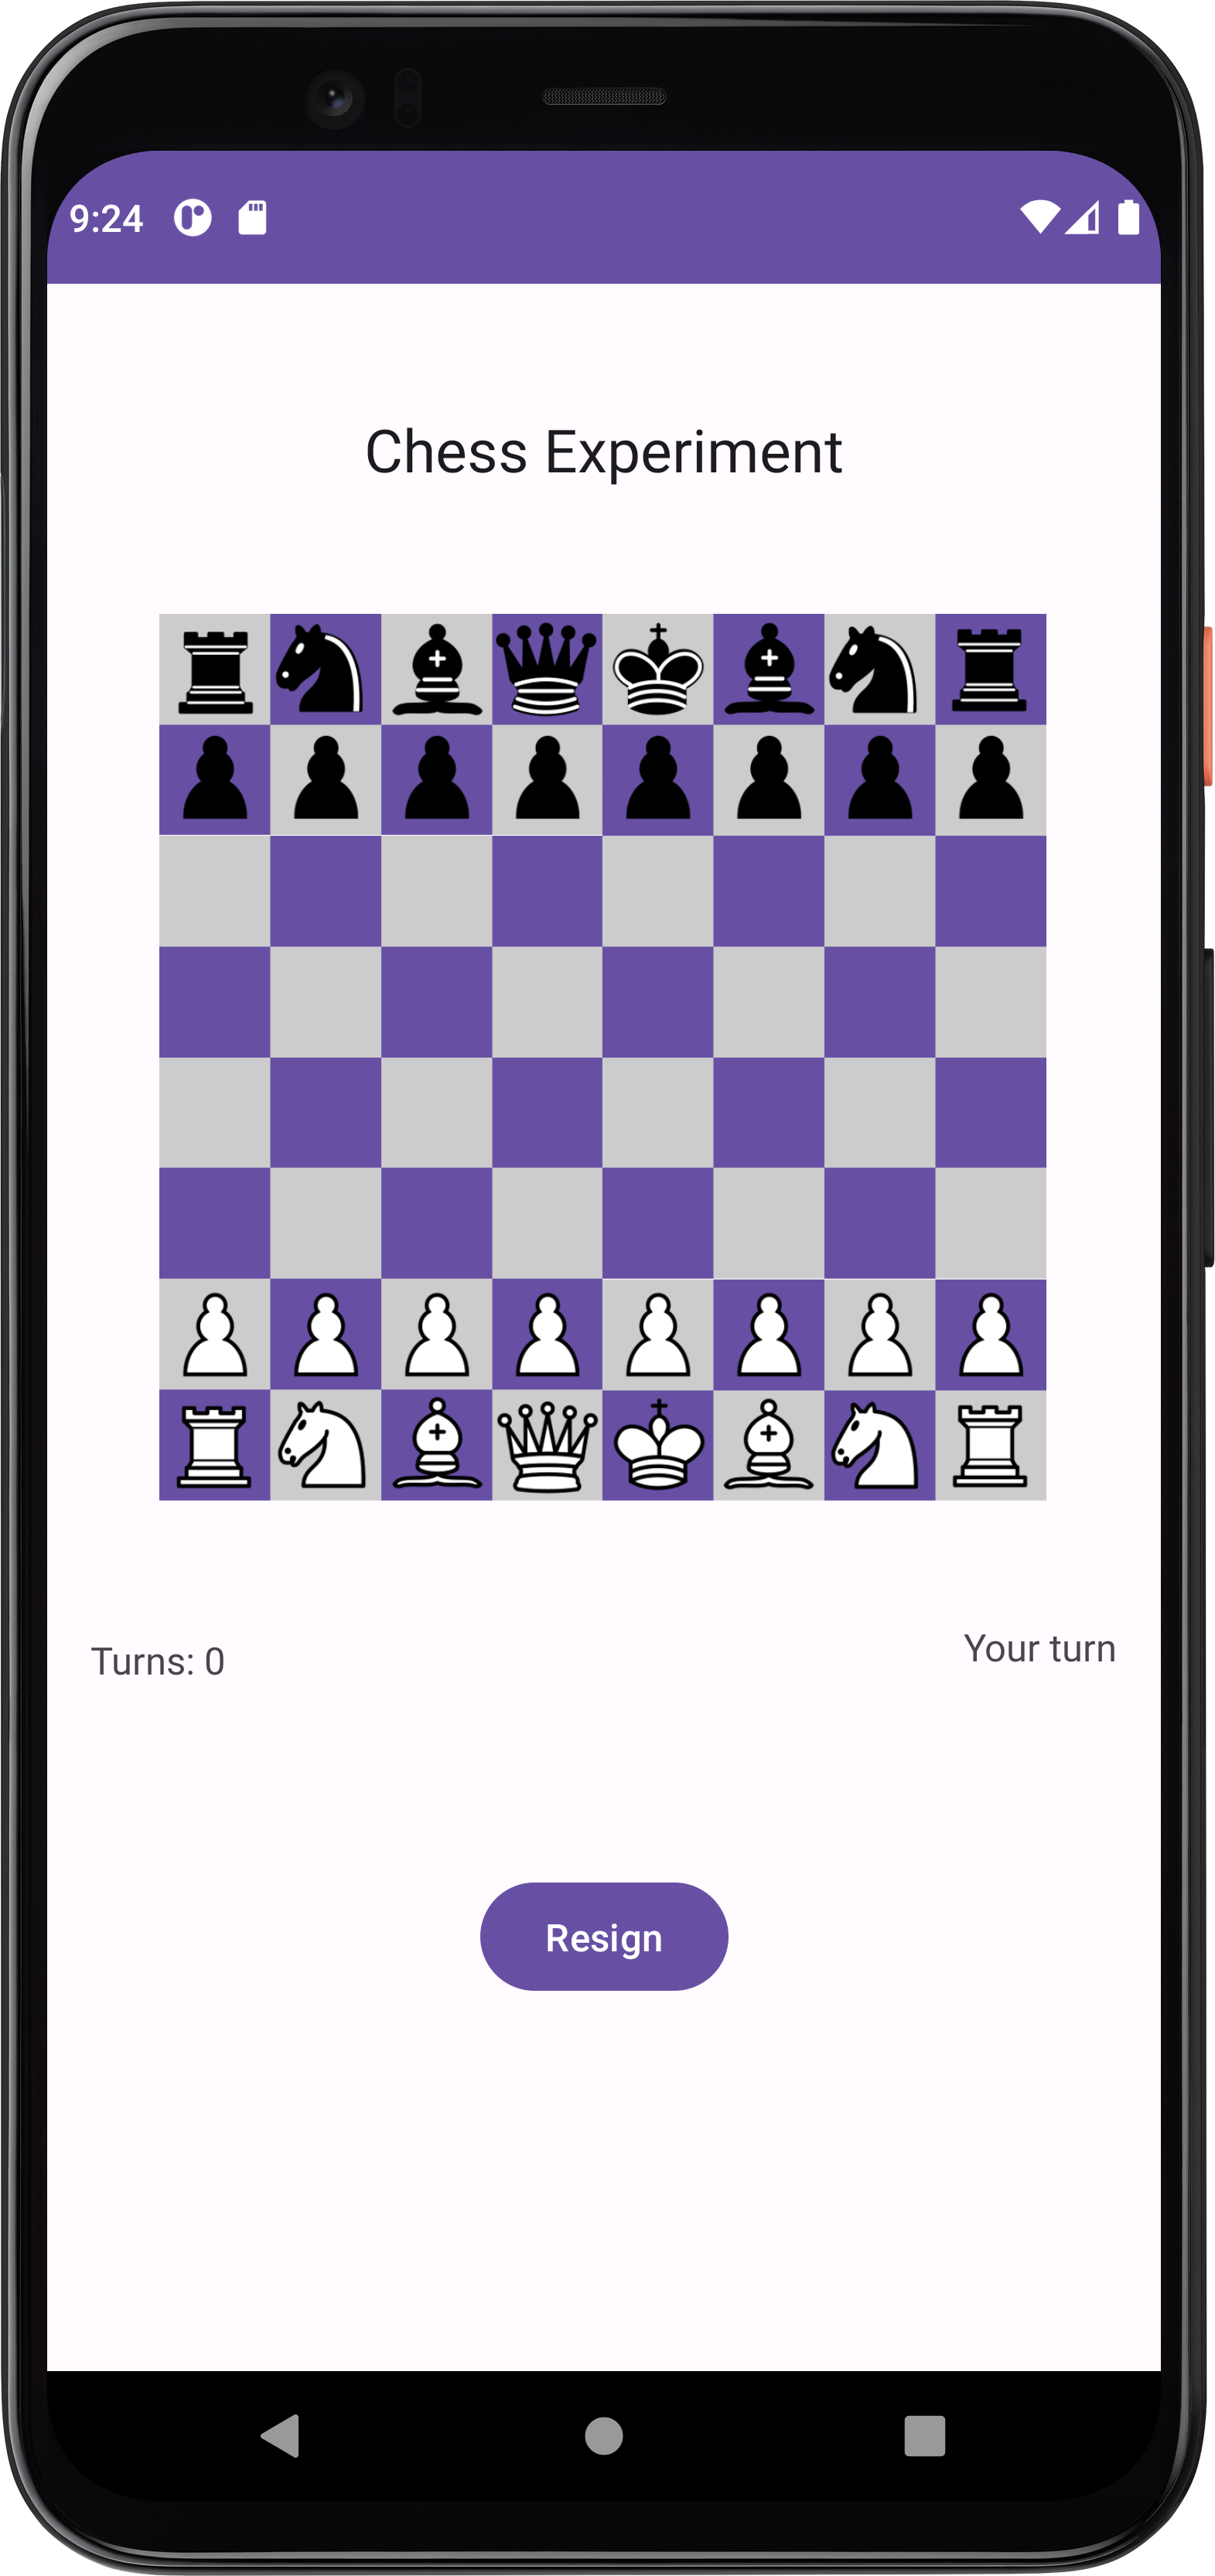
\includegraphics[width=0.3\textwidth, keepaspectratio]{content/07_evaluation_of_the_solution/Screenshot_Chess.png}
    \caption{Custom experiment logic}    
    \label{fig:chess}
\end{figure}

\newpage\subsubsection*{T6: Two groups are created, one of the groups is particularly chosen the other one randomly selected}

%the first one through putting the group into the respective participant data
%second through code within the use case:

\vspace{1cm}

\begin{lstlisting}[language=java,label=t3b,lineskip={0pt}, caption=Collect time needed to conduct experiment (b), basicstyle=\scriptsize, captionpos=b]
    currentParticipant = getCurrentParticipantUseCase.getCurrentParticipant();
    currentParticipantGroup = participantRepository.getParticipant(currentParticipant).getGroupAllocation();
    
    if(currentParticipantGroup == null){
    
        if(experimentRepository.getExperiment().getGroupAllocation() == "random"){
            Random random = new Random();
            int randomNumber = random.nextInt(2); // Generates either 0 or 1
    
            if(randomNumber == 0 ){
                setGroupAllocationPUseCase.setGroupAllocation("Group A", currentParticipant);
            } else {
                setGroupAllocationPUseCase.setGroupAllocation("Group B", currentParticipant);
            }
    
        };
    
    }
\end{lstlisting}

\newpage\subsubsection*{T7: A chess turn is played by both parties not using the same device}

\vspace{1cm}

\newpage\subsubsection*{T8 :The results of the experiment are retrieved and displayed in third party software}

\vspace{1cm}


\begin{lstlisting}[language=java,label=t3b,lineskip={0pt}, caption=Collect time needed to conduct experiment (b), basicstyle=\scriptsize, captionpos=b]
    File file = new File(Environment.getExternalStorageDirectory() + "/participant" + GetCurrentParticipantUseCase.getInstance().getCurrentParticipant() + "TimeData.csv");
    try {
        // create FileWriter object with file as parameter
        FileWriter outputfile = new FileWriter(file);

        // create CSVWriter object filewriter object as parameter
        CSVWriter writer = new CSVWriter(outputfile);

        // adding header to csv
        String[] header = { "id", "time in milliseconds"};
        writer.writeNext(header);

        //Getting participant information
        ArrayList<ParticipantEntity> participantEntities = GetParticipantDataUseCase.getInstance().getParticipantData();

        //Writing current participant time into file
        //String[] data = {String.valueOf(GetCurrentParticipantUseCase.getInstance().getCurrentParticipant()), String.valueOf(timeDifference)};


        Iterator iter = participantEntities.iterator();
        while (iter.hasNext()) {
            String[] data = {String.valueOf(((ParticipantEntity)iter.next()).getId()), String.valueOf(((ParticipantEntity)iter.next()).getExperimentTime())};
            writer.writeNext(data);
        }
        //closing writer connection
        writer.close();
    }
    catch (IOException e) {
        // TODO Auto-generated catch block
        e.printStackTrace();
        System.out.println("Error");
    }
\end{lstlisting}

\begin{figure}[htbp]
    \centering
    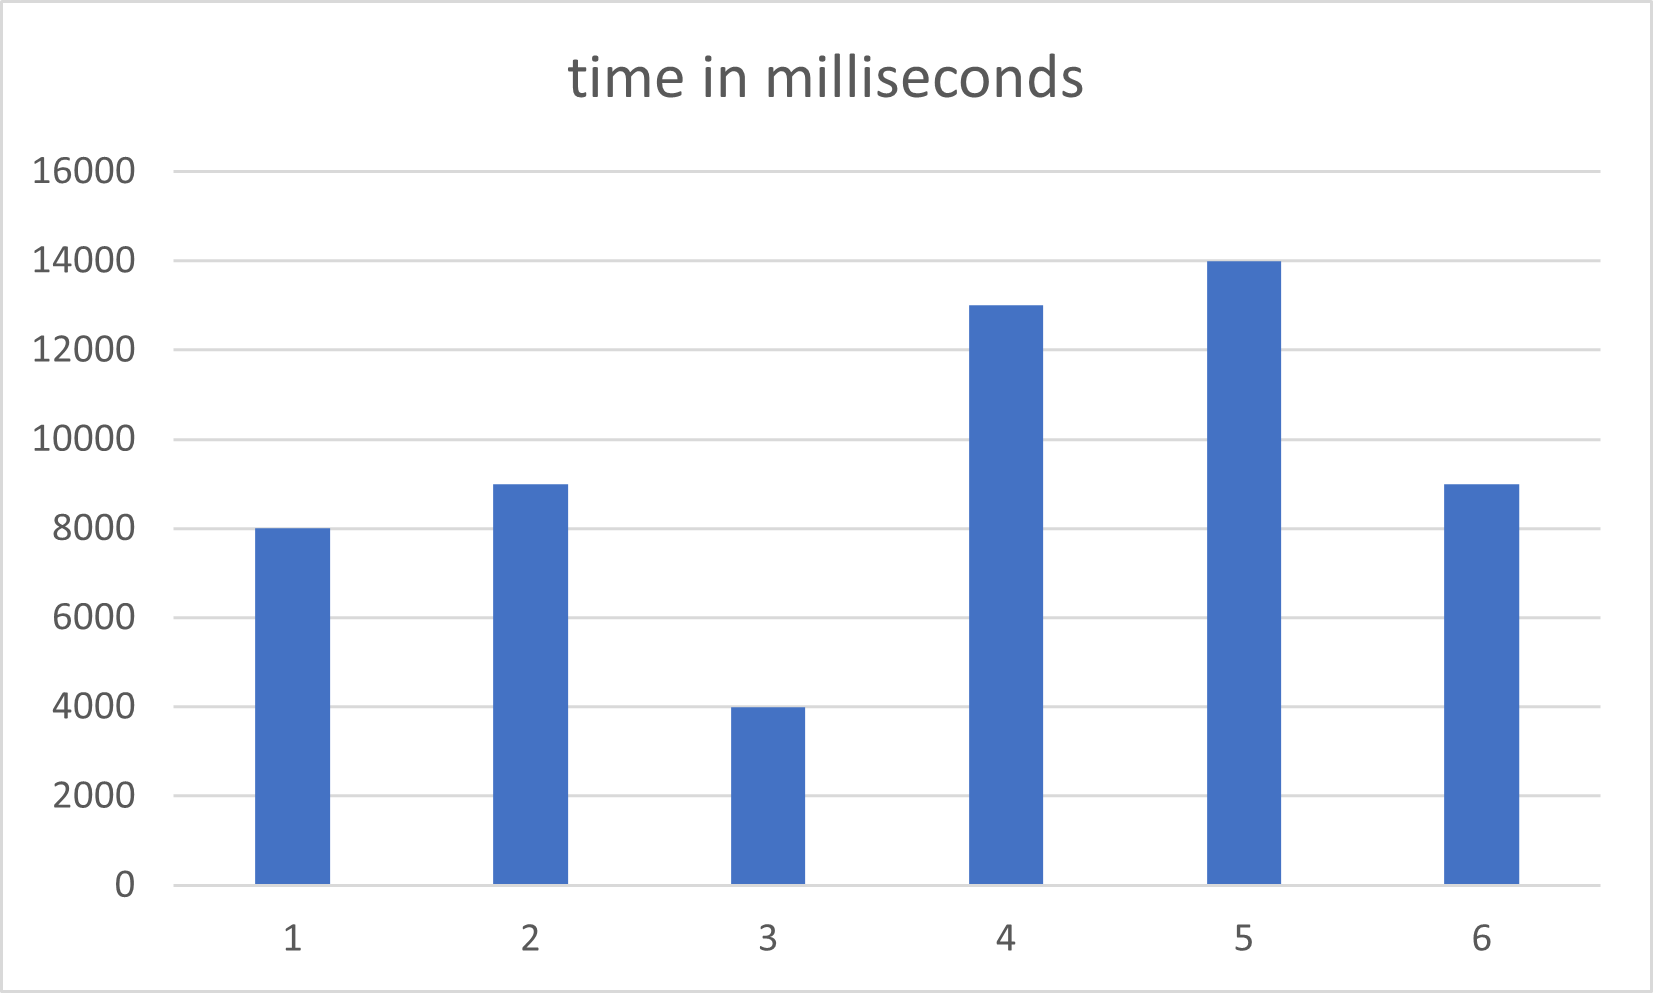
\includegraphics[width=0.25\textwidth, keepaspectratio]{content/07_evaluation_of_the_solution/ExcelPicture.png}
    \caption{Data loaded into excel}    
    \label{fig:Excel}
\end{figure}


\newpage\subsubsection*{T9: The experiment is redone a second time and another experimental setup is implemented}

%just change the experiment data

    %\begin{lstlisting}[language=java,label=t3b,lineskip={0pt}, caption=Collect time needed to conduct experiment (b), basicstyle=\scriptsize, captionpos=b]
    %ArrayList<String> steps = new ArrayList<String>();

    %steps.add("com.example.master_thesis.InfoScreenActivity");
    %steps.add("com.example.master_thesis.ChooseTestSubjectActivity");
    %steps.add("com.example.master_thesis.QuestionnaireActivity");
    %steps.add("com.example.master_thesis.ChessExperimentActivity");
%\end{lstlisting}

\vspace{1cm}

\newpage\subsubsection*{T10: The experiment is conducted on different devices}

%PIXEL 6 PRO API 30
\vspace{1cm}

\begin{figure}[htbp]
    \centering
    \begin{subfigure}[b]{0.25\textwidth}
        \centering
        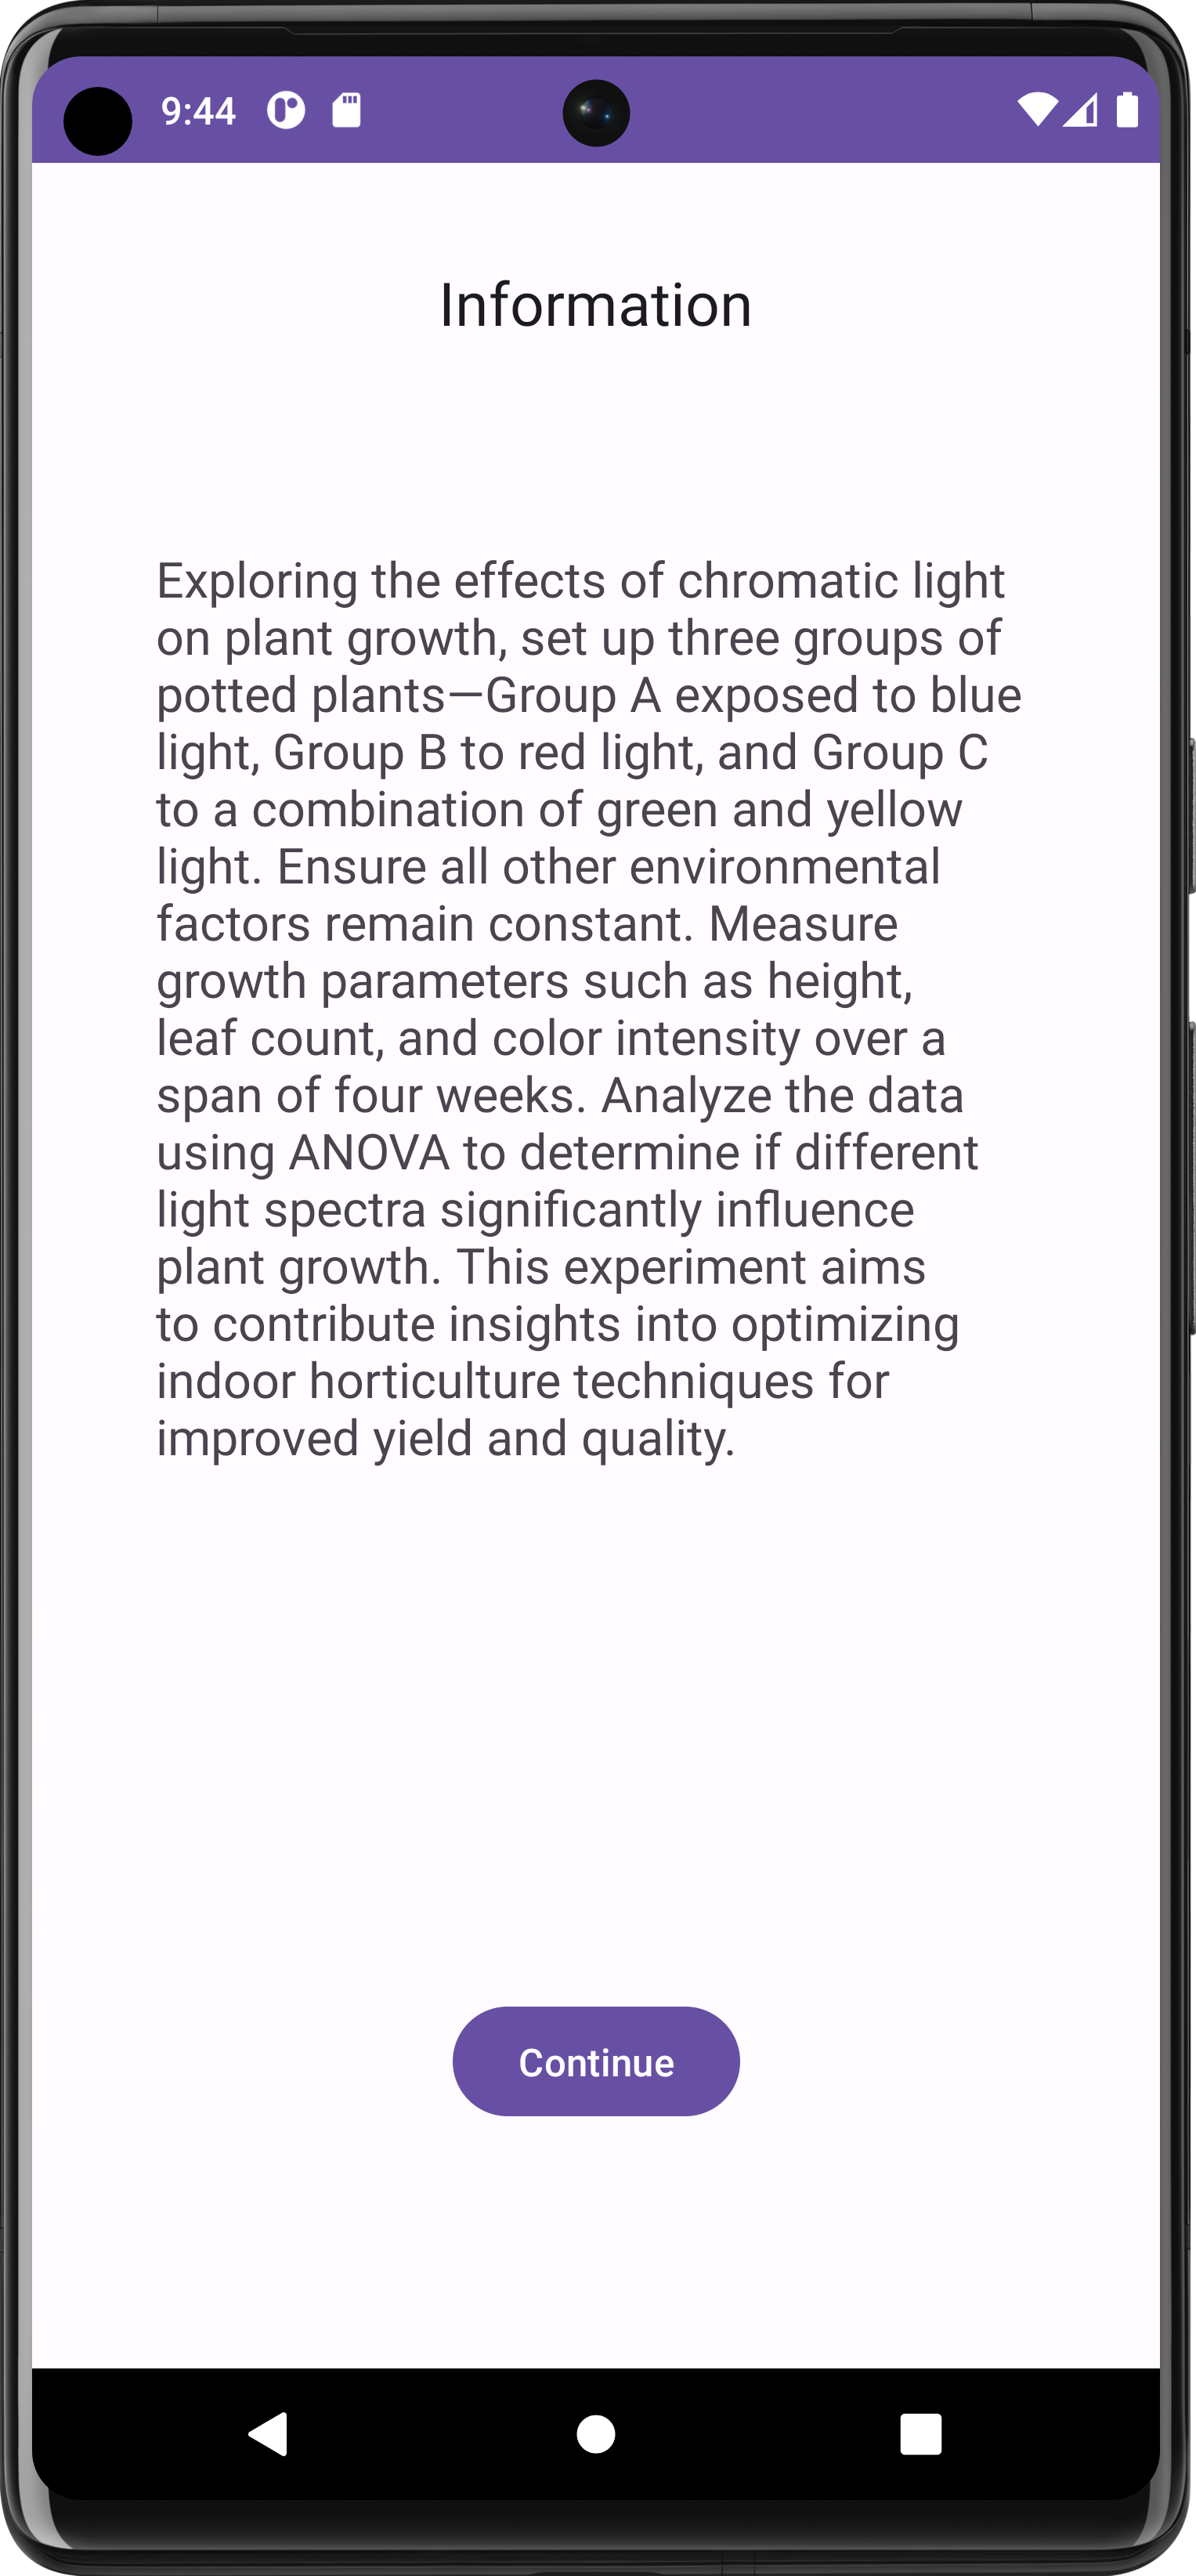
\includegraphics[width=\textwidth]{content/07_evaluation_of_the_solution/Screenshot_T10a.png}
        \caption{Info screen step | Pixel 6 Pro}
        \label{subfig:InfoScreenPixel}
    \end{subfigure}
        %\hfill
        \hspace{1cm}
    \begin{subfigure}[b]{0.25\textwidth}
        \centering
        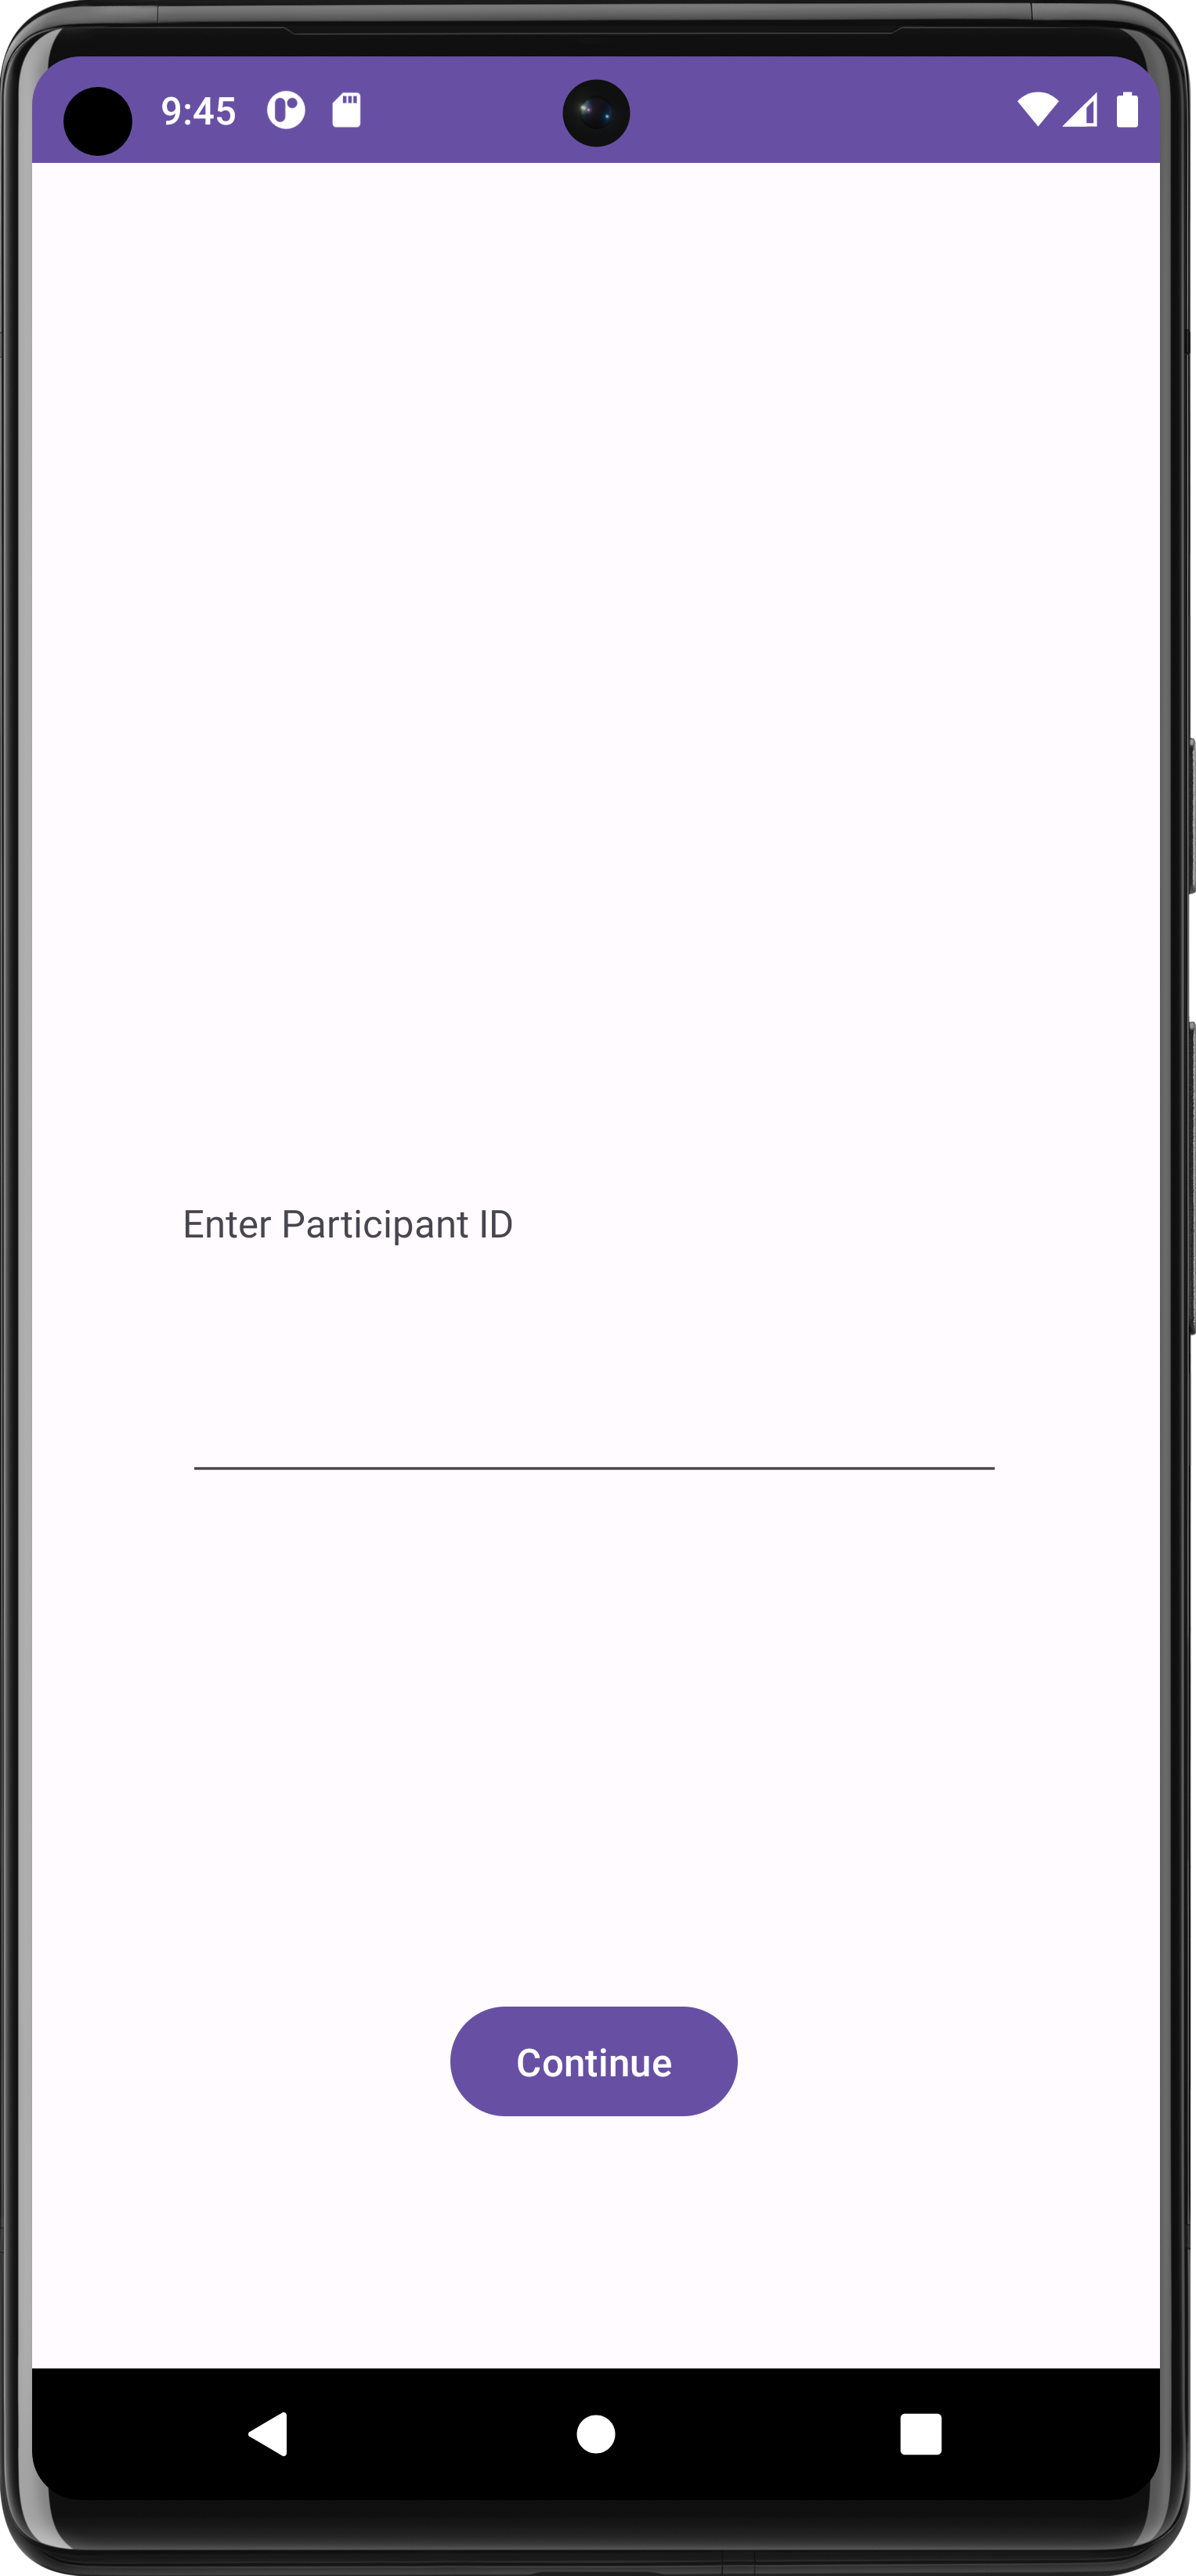
\includegraphics[width=\textwidth]{content/07_evaluation_of_the_solution/Screenshot_T10b.png}
        \caption{ Questionair step | Pixel 6 Pro}
        \label{subfig:QuestionairPixel}
    \end{subfigure}
        %\hfill
        \hspace{1cm}
    \begin{subfigure}[b]{0.25\textwidth}
        \centering
        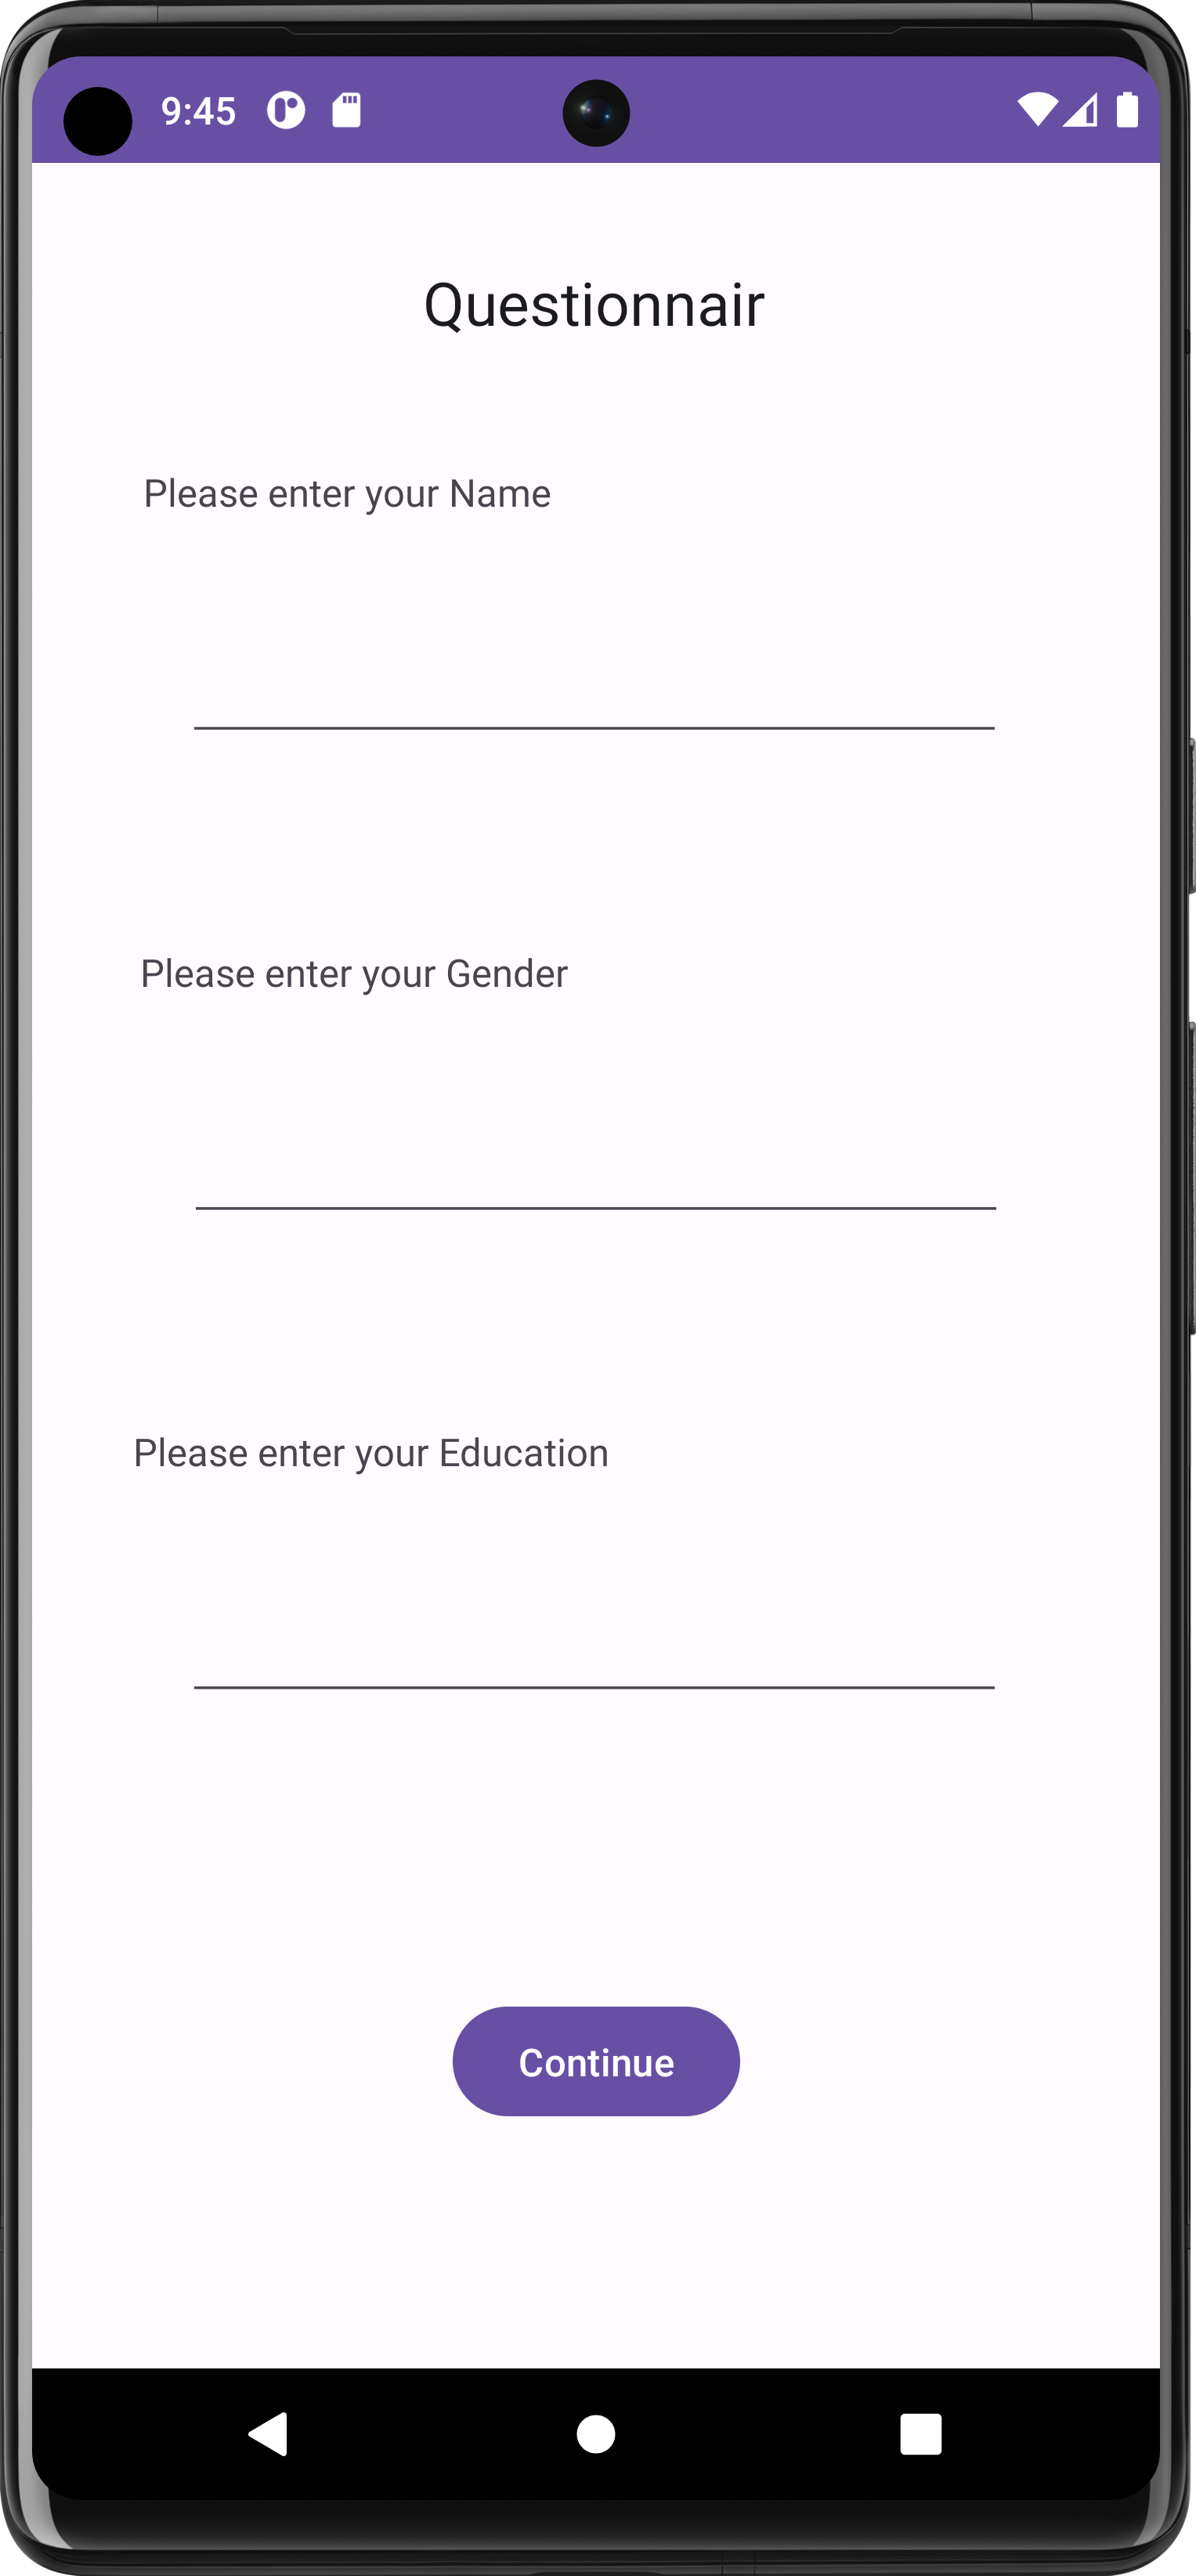
\includegraphics[width=\textwidth]{content/07_evaluation_of_the_solution/Screenshot_T10c.png}
        \caption{Choose test subject step | Pixel 6 Pro}
        \label{subfig:chooseTestSubjectPixel}
    \end{subfigure}
       \caption{Artefact run on a Pixel 6 Pro}
       \label{fig:uiScreens}
\end{figure}

\newpage\subsubsection*{T11: During the experiment the current state of the chess board is exported to the conducter of the experiment}

\subsubsection*{Remaining requirements}



%\subsection{Prototype Testing}



\subsection{App Performance and Usability}
